\chapter{Fundamentação teórica}

Este capítulo discorre sobre os tópicos, tecnologias e técnicas empregadas no desenvolvimento do trabalho.

\section{Análise de dados}

Com a produção de dados dos mais variados contextos é comum que pessoas com interesse nesses dados passem a agrupar, ordenar e tentar buscar informações que remetam a respostas de problemas ou dúvidas inerentes aos dados. O processo de Análise de Dados (AD) pode ser definido como "a execução de técnicas e etapas para a extração de um conhecimento agregado no contexto de um conjunto de dados" \cite{AMARAL2016}. \citeonline{KRATOCHWILL2015} o definem como um método onde quem faz a análise pode elaborar conclusões ou levantar hipóteses sobre o relacionamento ou falta deste para o conjunto de informações analisadas.

A execução de análise sobre dados não precisa envolver técnicas modernas ou passos complexos. Na realidade, a análise de dados pode ser feita com uma simples ordenação de uma coluna de uma planilha excel ou mesmo em uma consulta SQL (\textit{Structured Query Language}) em uma base de dados relacional \cite{AMARAL2016}. 

A aprendizagem de máquina (\emph{machine learning}) fornece a base técnica para as análises de dados mais complexas. É utilizada para extrair informações de dados brutos, onde os resultados podem ser utilizados para diversos fins \cite{Witten2016}. Em um contexto mais amplo, as técnicas relacionadas ao aprendizagem de máquina ajudam a encontrar informações difíceis de serem observadas por técnicas mais simples (como a ordenação ou a consulta simples).

Sabendo que a partir da análise de dados é possível obter respostas mais elaboradas, a sua utilização vem crescendo em muitas áreas do conhecimento, como a área da Medicina \cite{Holzinger2014}. A análise de dados pode utilizar técnicas como o Knowledge Discovery in Databases (KDD) \cite{Holzinger2014} e Mineração de dados \cite{Aggarwal2015} para entregar resultados mais precisos.

Podemos imaginar que os trabalhos que envolvem a AD tem como objetivo final a criação de ferramentas ou relatórios que serão úteis para demonstrar comportamentos relevantes e não triviais do conjunto de dados com o intuito de prover um melhor entendimento do problema observado. No entanto é válido frisar que todo este processo pode ser complexo e demorado. Os próximos tópicos mostrarão de forma mais aprofundada as técnicas comumente empregadas para realizar a análise de dados e como os resultados podem ser apreciados.

\section{\emph{Knowledge Discovery in Databases}}

Na área da Medicina e da Informática é relativamente fácil produzir quantidades de dados que excedem gigabytes de armazenamento \cite{Holzinger2014}. Tais informações podem vir de fontes diversas, como resultados de estudos científicos, observações empíricas digitalizadas, websites ou até mesmo da coleta de informações sobre pacientes em prontuários. O armazenamento de dados com fontes tão variadas pode se tornar complexo, já que é comum obtermos dados que são estruturados (e.g., dados de tabelas em um banco Relacional), semi-estruturados (e.g., dados em documentos XML), dados que não possuem nenhum tipo de estrutura (e.g., arquivo de texto plano), dados incompletos ou até mesmo fora de contexto e que podem ser considerados como ruídos durante uma futura análise.

A busca de informações em bancos de dados de forma pragmática pode ser tomada como um meio não só de extração de informações significantes mas também como uma maneira de adquirir conhecimento, conhecimento este que antes era impensável ou até mesmo distante.

O grande desafio de se trabalhar com informações de fontes diferentes se dá desde a coleta dos dados até a fase de exploração. É necessário que etapas sejam definidas de modo que possam ser reproduzidas e aprimoradas no decorrer do seu processo.

O \emph{Knowledge Discovery in Database} (KDD) é um processo de descoberta de conhecimento a partir de uma coleção de dados, constituído por várias etapas, de maneira interativa e iterativa, para identificação de padrões compreensíveis, válidos e potencialmente úteis \cite{Fayyad1996}. As etapas do KDD são: seleção dos dados, pré processamento, transformação dos dados, mineração de dados e interpretação dos resultados \cite{Holzinger2014, Fayyad1996}. A Figura \ref{fig:kdd} demonstra estas etapas e o fluxo do processo. A seguir detalhamos cada uma das etapas indicadas.

\begin{figure}[htb]
  \caption{\label{fig:kdd}Etapas do KDD}
  \begin{center}
    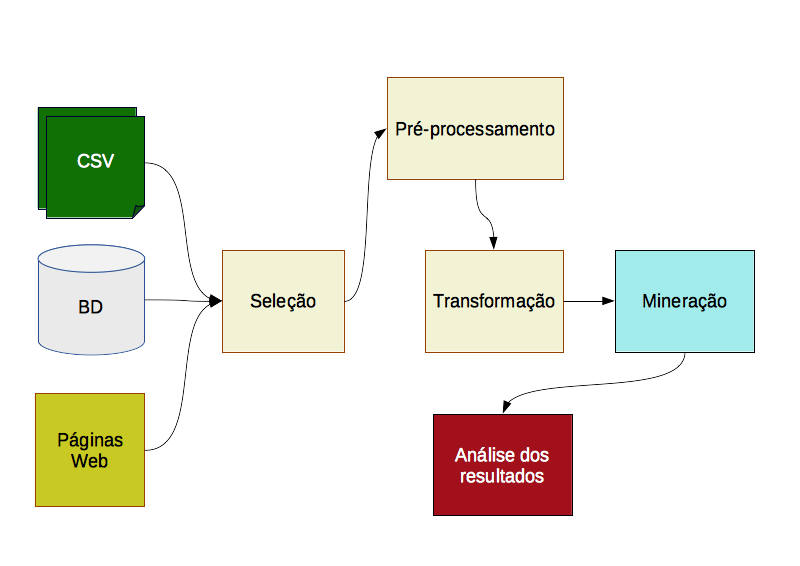
\includegraphics[scale=0.8]{imagens/kdd.png}
    \legend{Fonte: Baseado em \citeonline{Silva2010}}
  \end{center}
\end{figure}
\newpage

% ---
% Início das etapas
\subsection{Seleção dos dados}

O processo de KDD é iniciado pela etapa de seleção de dados. Este é um passo demorado e, muitas vezes, complexo, visto que um projeto pode utilizar uma ou mais fontes de dados para a seleção, e o que será coletado durante esta etapa também vai variar de acordo com o contexto do projeto. É comum que as informações a serem coletadas sejam escolhidas por um especialista no domínio do problema \cite{Boente2008}. A seleção de dados, muitas vezes, se depara com fontes que apresentam os seus dados de forma semiestruturada ou não estruturada. Neste sentido é necessário criar programas ou utilizar ferramentas que auxiliem, de maneira prática, o acesso, captura e armazenamento das informações.

É comum utilizarmos linguagens de programação para a criação de scripts que automatizam o trabalho de seleção, a exemplo da linguagem Python\footnote{\url{https://www.python.org}} \cite{Smedt2012}. Também podemos utilizar a linguagem SQL para a extração de informações já estruturadas em bases de dados consolidadas. Fica evidente, então, que esta etapa poderá utilizar uma ou mais ferramentas para a sua execução.

\subsection{Pré-processamento}

Em posse das informações coletadas na etapa anterior, a etapa de  pré-processamento é iniciada. Esta é uma etapa muito importante no processo KDD, visto que é comum realizarmos ajustes no conjunto de dados, que visam melhorar a qualidade das informações coletadas \cite{Aggarwal2015}. Ilustrações de tarefas de pré processamento são a remoção de dados redundantes e inconsistentes, identificação e avaliação de dados discrepantes, tratamento de dados ausentes, normatização para formatos de datas e obtenção de informações a partir de outras características como, por exemplo, a obtenção de idades de pessoas a partir de datas de nascimento ou nome de cidades por meio do código de endereçamento postal (CEP).

\subsection{Transformação}

Logo após a seleção e pré processamento dos dados, é preciso transformar o resultado de maneira que as informações fiquem padronizadas para consultas posteriores. Esta etapa representa a consolidação dos últimos dois passos. Para que os algoritmos de mineração possam trabalhar em cima dos dados é necessário que durante a etapa de transformação os dados como um todo sejam convertidos para o formato adequado de acesso.

O armazenamento de dados normalmente é feito em um SGBD (Sistema gerenciador de banco de dados), mas também é possível encontrá-los  em arquivos tabulares como, por exemplo, em arquivos CSV\footnote{Formato de arquivo texto comumente empregado utilizado para a troca de dados entre aplicações, no qual cada linha corresponde a um registro e os campos são separados entre si por vírgula.} (\emph{Comma-Separated Values}). Dependendo da ferramenta utilizada para a análise dos dados, é possível que o armazenamento em um SGBD ou em arquivos CSV não seja suficiente.

Ferramentas como o Weka \cite{Hall2009} e Tensorflow\footnote{\url{https://www.tensorflow.org}} utilizam formatos de arquivos personalizados para a realização do trabalho de mineração. No caso do Weka o formato de arquivo é o \emph{Attribute-Relation File Format} (ARFF)\footnote{\url{https://www.cs.waikato.ac.nz/ml/weka/arff.html}}, que na sua estrutura possui uma maneira própria para determinar os atributos e tipos de dados contidos. Sendo assim é possível que o formato de armazenamento e consolidação dos dados varie de acordo com a ferramenta escolhida para as etapas de análise.


\subsection{Mineração de dados}

Mineração de dados é um processo automático ou semi automático que, por meio de técnicas de exploração, busca a extração de novos padrões potencialmente úteis em grandes quantidades de dados, de modo que estes padrões não seriam facilmente descobertos a olho nu \cite{Fayyad1996,Witten2016}. O grande desafio nesta etapa é que cada conjunto de dados é único, ou seja, as suas características de formatação, armazenamento e representação de informação pode variar bastante e isto dificulta a criação de ferramentas que possam ser reutilizadas em contextos diferentes. Também é possível categorizar  as tarefas de exploração dos dados como supervisionadas e não supervisionadas \cite{Aggarwal2015}. O processo de mineração de dados pode ser dividido em quatro tipos de tarefas: associação de regras, classificação, agrupamento em conjuntos e  detecção de outliers \cite{Aggarwal2015}. Quando estamos tentando definir o valor (por discriminação ou categorização) de uma coluna especial em um \emph{dataset} nós estamos trabalhando com uma tarefa de classificação.

A classificação tem o objetivo de atribuir um rótulo para uma ou mais instâncias de um \emph{dataset} de modo que esta atribuição seja feita por meio da análise prévia de características de outras instâncias similares. Um exemplo prático pode ser visto com a classificação de doenças em níveis de intensidade (classes), onde o classificador irá se basear em dados de um \emph{dataset} como os sintomas (atributos) de cada instância da doença para formar um conhecimento que será utilizado para predizer o nível de uma nova instância de doença ainda não conhecida dentro do \emph{dataset}.

A tarefa de classificação é considerada como uma tarefa de aprendizagem supervisionada, já que é preciso apresentar ao algoritmo de aprendizagem informações o conjunto de valores dos atributos e sua respectiva classe. Do outro modo nós temos as tarefas de agrupamento, regra de associação e detecção de \emph{outliers} que são consideradas como tarefas de aprendizagem não supervisionadas, já que não são apresentadas ao algoritmo de aprendizagem informações para "ensinar" como a tarefa será executada perante os dados em questão \cite{Aggarwal2015}.

Este trabalho utiliza as técnicas de classificação e por isso estas serão apresentadas em detalhes na seção 2.3.


\subsection{Interpretação dos resultados}

Logo após a mineração dos dados, entramos na fase de interpretação e avaliação dos resultados obtidos.  É comum que nesta etapa os resultados da mineração sejam avaliados por um especialista no domínio do problema a fim de corroborar o conhecimento que foi minerado a partir dos dados brutos. Esta é uma fase que tende a ser realizada várias vezes durante um mesmo projeto pois é normal que as informações encontradas não sejam precisas o suficiente ou não façam sentido para o contexto do projeto nas primeiras iterações. O especialista do domínio assiste a esse processo e ajuda a reinicializar todo o processo de KDD ou parte dele sempre que necessário. Desta forma é possível que os dados e características selecionadas na primeira etapa sofram modificações, assim como a etapa de mineração de dados em si com o algoritmo escolhido para tal.

\section{Técnicas de Classificação}
Existem inúmeras técnicas de mineração descritas na literatura, muitas remetem aos quatro grande tarefas apresentados na seção anterior. Este tópico tem como intuito apresentar algoritmos de aprendizagem utilizados em técnicas de classificação, suas limitações e seus principais casos de uso.

Os algoritmos de aprendizagem de máquina podem ser chamados de classificadores quando a tarefa a ser executada é de classificação. Um classificador pode ser entendido como uma função que recebe informações de entrada e, a partir do processamento dessas informações, produz uma saída conhecida como modelo \cite{Fayyad1996}. Este processo é conhecido como treinamento.

O classificador pode trabalhar com tarefas onde as opções de classes para treinamento e predição variam entre duas ou mais, desta maneira a tarefa de classificação pode ser binária ou multiclasse (ou multinomial) \cite{Aggarwal2015}.

A classificação binária remete à tarefa onde o algoritmo precisa aprender sobre duas classes, normalmente nomeadas como   Positiva e Negativa. Um exemplo de classificação binária é quando o algoritmo precisa determinar se um paciente está ou não com uma doença específica. Já um problema multiclasse remete à tarefa onde o algoritmo precisa aprender sobre como classificar uma instância mediante a escolha entre três ou mais opções de classes. Classificar uma doença por meio de vários níveis de risco é uma tarefa de classificação multiclasse.

Os modelos de classificação são produzidos a partir de informações estatísticas, lógicas e padrões resultantes do processamento dos dados de entrada\footnote{\url{https://docs.microsoft.com/en-us/sql/analysis-services/data-mining/mining-models-analysis-services-data-mining}}, e estes dados são as instâncias de um \emph{dataset}, onde cada instância é composta por um conjunto de valores relacionados aos atributos. É possível utilizar a mesma fonte de dados para treinar vários modelos diferentes de classificação. Algoritmos como Naive Bayes \cite{Mccallum1998}, \emph{Support Vector Machines} (SVM) \cite{Meyer2017} e árvores de decisão \cite{Schmid2013} resultarão em modelos distintos, cada um com suas características, pontos fortes e fracos. A escolha de qual algoritmo utilizar vai depender, por exemplo, do contexto do problema, tamanho do \emph{dataset} e nível de desbalanceamento das classes (desproporção entre o número de exemplos de cada classe).

Antes da criação de um modelo de dados é preciso selecionar quais instâncias de um \emph{dataset} serão utilizadas para treinamento do algoritmo. Existem técnicas específicas para esta necessidade, sendo as mais conhecidas: a \emph{holdout} e a \emph{k-fold Cross-validation} \cite{Kohavi1995}.

O método \emph{holdout} é o mais simples dos dois mencionados, pois consiste em segmentar o \emph{dataset} em subconjuntos de treino e de teste, onde os segmentos são mutuamente excludentes. Historicamente são utilizadas as proporçòes de $\frac{2}{3}$ do \emph{dataset} para treino e de $\frac{1}{3}$ para teste \cite{Kohavi1995}.

Um dos problemas do método \emph{holdout} é que normalmente a seleção das instâncias se torna enviesada se as classes estiverem em desproporção nas partições ou se a forma de seleção das instâncias não for feita de uma maneira aleatória e sem repetição. É comum que as partições dos conjuntos de treino e teste sejam feitas com um método chamado de estratificação, onde a estratificação é responsável por montar os grupos com a seleção aleatória das instâncias a partir do \textit{dataset}, mantendo-se a mesma proporção de instâncias de cada classe em cada partição. Desta forma a seleção das instâncias não segue uma sequência linear e os grupos podem manter a proporção de instâncias.

Levando em consideração um \emph{dataset} que possui a mesma quantidade de elementos para duas classes diferentes e, se o holdout utilizado não for estratificado, a partição de treino é realizada na proporção de $\frac{2}{3}$. Esta, por sua vez, possuirá mais elementos de uma classe do que de outra o que poderá afetar no resultado do treinamento \cite{Witten2016}.

O método \emph{k-fold} consiste em segmentar o conjunto de dados em K grupos (\emph{folds}) mutuamente excludentes, onde o treinamento do algoritmo será feito com k-1 \emph{folds} e o \emph{fold} restante será utilizado para teste, havendo um rodízio na formação dos conjuntos de treino e testes para garantir que todos os grupos participem do conjunto de treino e de testes. \citeonline{Kohavi1995} demonstra que a escolha de $k = 10$ é razoavelmente adequada para a grande maioria dos problemas, visto que os acertos da classificação não são melhorados de forma significativa para grandes valores de K, o que não justificaria o esforço computacional utilizado para o treinamento.

É necessário observar que o método \emph{k-fold} é computacionalmente mais caro que o método \emph{Holdout} já que o algoritmo será treinado k vezes, contudo esta abordagem diminui o viés dos dados entregues para o algoritmo de treinamento e diminui a variância das medidas de avaliação, o que, consequentemente gera melhores resultados de classificação \citeonline{Kohavi1995}.


\section{Ferramentas de Suporte à Análise de Dados}

A partir da evolução da Computação e da popularização da Ciência de Dados, ferramentas cada vez mais completas tem sido criadas para oferecer o suporte necessário para as etapas da análise de dados. Atualmente algumas das ferramentas mais utilizadas para este fim são a Weka \cite{Hall2009}, a linguagem de programação R\footnote{\url{https://www.r-project.org}} e a linguagem de programação Python\footnote{\url{https://www.python.org}}.

\subsection{Weka}

Segundo \citeonline{Frank2016}, Weka é uma coleção de algoritmos de aprendizagem de máquina para tarefas de mineração de dados. Os algoritmos podem ser aplicados diretamente a um \textit{dataset} usando a interface do Weka Explorer ou podem ser invocados a partir de um código Java\footnote{\url{https://www.java.com/}} (Weka API - Application Programming Interface). Weka provê suporte para tarefas de  pré-processamento, classificação, regressão, regras de associação e visualização de resultados. A ferramenta Weka foi escrita na linguagem  Java. Diferentemente do Python e R, o Weka oferece uma interface gráfica pronta para uso, assim é possível realizar todas as operações da mineração de dados por meio desta interface (Figura \ref{fig:weka}).

\begin{figure}[htb]
  \caption{\label{fig:weka}Weka GUI Interface}
  \begin{center}
    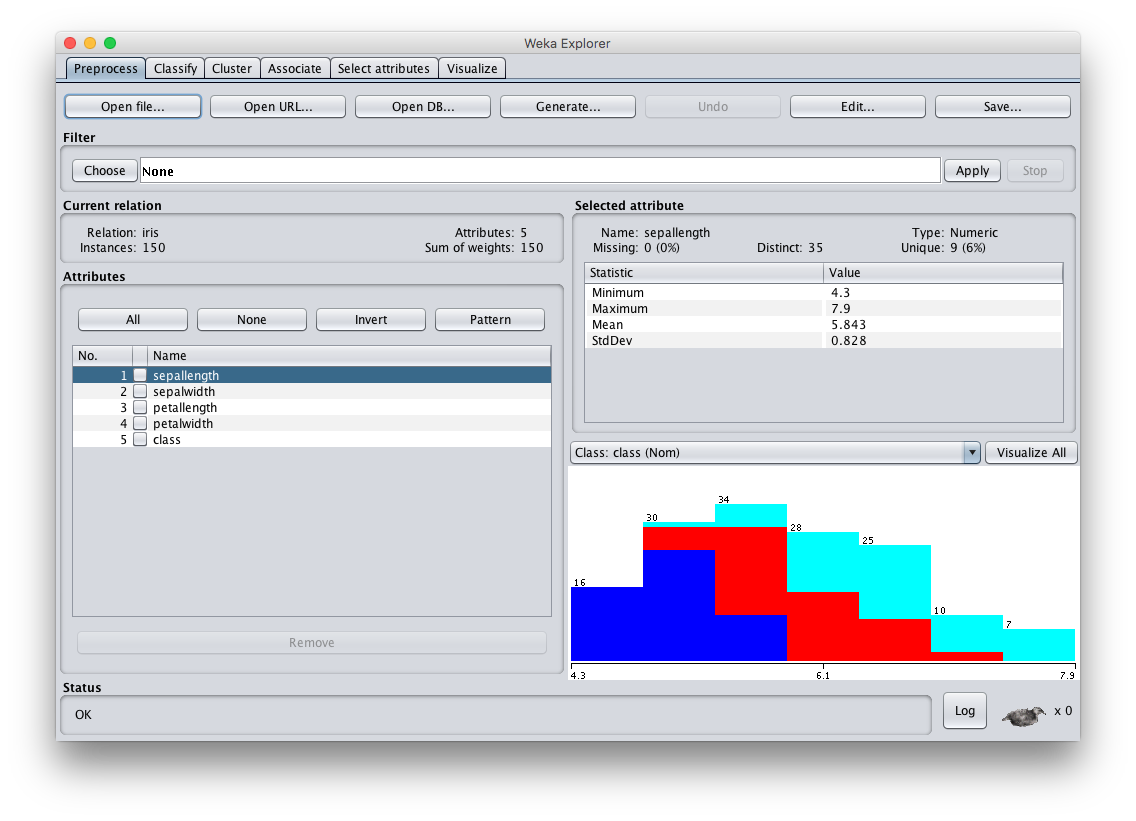
\includegraphics[scale=0.4]{imagens/weka.png}
    \legend{Fonte: \citeonline{Hall2009}}
  \end{center}
\end{figure}
\newpage

A Figura \ref{fig:weka} exibe a interface gráfica da ferramenta Weka, onde é possível ver os menus disponíveis para realizar as tarefas de classificação,  agrupamento e associação. Figura \ref{fig:weka} também exibe as informações sobre o \textit{dataset} e seus atributos.

\subsection{Linguagem R}
R é um software livre que combina um linguagem de programação e um ambiente de desenvolvimento integrado para a realização de cálculos estatísticos, visualização de gráficos e execução de rotinas de código armazenadas em \textit{script} \cite{Team2018}.

A linguagem disponibiliza um REPL (\textit{read-eval-print-loop}) para a execução de comandos de maneira rápida e fácil, sendo possível criar e invocar funções, criar e carregar \textit{datasets} e criar e carregar modelos estatísticos. Por se tratar de um software \textit{open source}\footnote{\url{https://opensource.org}}, R conta com uma quantidade expressiva de colaboradores, estes, por sua vez, disponibilizam extensões para o ecossistema da linguagem. R também conta com um grupo de desenvolvedores dedicados para a linguagem desde 1997, o que traz mais segurança para que mais pessoas e empresas invistam na sua utilização.


\subsection{Python}

Python é uma linguagem de programação interpretada de propósito geral, imperativa, orientada a objetos, funcional, de tipagem dinâmica e forte\footnote{\url{https://www.python.org/doc/essays/blurb/}}. É  linguagem de alto nível que é fundamentada na priorização do esforço do programador acima do esforço computacional.

Diferentemente do Weka e da linguagem R, Python não foi criada com o intuito de servir à computação estatística e gráfica, porém, por sua capacidade de extensão, os desenvolvedores colaborativos criaram módulos que conversam com outras linguagens de programação como FORTRAN\footnote{\url{https://web.fe.up.pt/~aarh/pc/PC-capitulo2.pdf}} e C\footnote{\url{https://docs.python.org/2/extending/extending.html}} o que tornou possível a criação de algoritmos eficientes para a análise de dados. Atualmente é possível encontrar muitos módulos para a análise de dados e visualização dos resultados para Python.

\section{Métricas para Avaliação}

Mensurar o desempenho de um algoritmo durante o processo de mineração é de suma importância. É preciso estabelecer métricas e parâmetros reproduzíveis para que haja a comparação de resultados entre diferentes algoritmos. É por meio das métricas de avaliação que poderemos analisar e ter \textit{insights} sobre os dados, ou seja, saberemos quais algoritmos possuem melhor desempenho para o caso em questão.

As medidas de \textit{precision} (precisão), \textit{recall} (\textit{sensitivity}, sensitividade ou cobertura) e \textit{f-measure} (média harmônica) são comumente empregadas para avaliar o desempenho de algoritmos de classificação \cite{Powers2011}. A especificidade  (\textit{specificity} ou  \textit{inverse-recall}) também pode ser utilizada.

\subsection{Matriz de confusão}

A matriz de confusão não é um método propriamente dito para medição do desempenho de um algoritmo de classificação, contudo, auxilia na visualização da classificação \cite{Deng2016} e entendimento do comportamento do classificador. A matriz gera uma tabulação com as informações sobre a classificação, dessa forma fica mais fácil analisar qual foi o comportamento da mineração.

Para entender a saída de dados da matriz de confusão é preciso conhecer o significado das siglas apresentadas na Tabela 1, estas são: Verdadeiros Positivos (TP), Falsos Positivos (FP), Verdadeiros Negativos (TN) e Falsos Negativos (FN) \cite{Powers2011}, vale lembrar que após a classificação os termos serão substituídos por números que representam as instâncias classificadas.

A Tabela \ref{tab:confusion} é um exemplo de uma matriz de confusão para a classificação com duas classes de exemplo, uma positiva e outra negativa. O parâmetro TP representa a quantidade de verdadeiros positivos que foram classificados corretamente para a  classe positiva, o parâmetro TN representa a quantidade de verdadeiros negativos que foram classificados corretamente para a classe negativa. O parâmetro FP representa a quantidade de instâncias que foram classificadas incorretamente para a classe positiva (foram classificadas como positiva mas eram da classe negativa) e o parâmetro FN representa a quantidade de instâncias que foram classificadas incorretamente para a classe negativa (foram classificadas como negativa mas eram da classe positiva) \cite{Powers2011}.

\begin{table}[h]
	\caption{\label{tab:confusion}Matriz de confusão}
	\begin{center}
	\begin{tabular}{c|c}
		\hline 
		\textbf{TP} & FN \\ 
		\hline
		FP & \textbf{TN} \\ 
		\hline 
	\end{tabular} 
	\legend{Fonte: O autor}
	\end{center}
\end{table}

Logo após gerarmos a tabulação com as informações sobre a classificação, é  interessante calcular o quão eficiente foi o treinamento. A partir desse momento levamos em consideração pelo menos três métricas utilizadas na recuperação de informação \cite{Buttcher2016} para realizar a avaliação do algoritmo de aprendizagem: \textit{Recall}, \textit{Precision}, \textit{Specificity}.

\textit{Precision} (precisão) é a proporção de casos preditos como positivos e que são de fato reais positivos, sendo assim estamos medindo a capacidade do algoritmo em classificar as instâncias do \textit{dataset} corretamente para a classe positiva.

\begin{equation}
Precision  = \frac{TP}{TP + FN}
\end{equation}

\textit{Recall} (\textit{sensitivity}) é a proporção de casos que são reais positivos e que foram corretamente classificados como tal, ou seja, estamos medindo a capacidade do nosso algoritmo de classificar os verdadeiros positivos para um conjunto de dados.

\begin{equation}
Recall  = \frac{TP}{TP + FP}
\end{equation}


A \textit{Specificity} (especificidade) é a proporção de casos preditos como negativos e que são de fato reais negativos. Com esta métrica nós estamos analisando a capacidade do algoritmo em prever os casos ditos reais negativos (TN). Diferentemente do \textit{Precision} e \textit{Recall}, quando a \textit{Specificity} é analisada, a intenção é focar na classificação dos ditos casos negativos, visto que em determinados casos como na Medicina é importante validar os casos que são verdadeiros negativos (pessoas que não possuem uma doença por exemplo) \cite{Holzinger2014}.

\begin{equation}
Specificity  = \frac{TN}{TN + FN}
\end{equation}

Quanto maior a proporção para estes três casos, melhor o algoritmo teria se saído durante a classificação. Por fim, podemos calcular a \textit{Balanced Accuracy} (Precisão balanceada) para a nossa matriz de confusão, que nos dará a média entre as proporções de casos verdadeiros positivos e verdadeiros negativos.

\begin{equation}
Balanced Accuracy  = \frac{Recall + Specificity}{2}
\end{equation}

\textit{F-measure}, ou como às vezes é chamada \textit{F-score}, é a média ponderada do \textit{Recall} e \textit{Precision}. É uma função herdada da Recuperação de Informação (\textit{Information Retrieval}) onde o \textit{Recall} é a frequência em que documentos relevantes são selecionados por um sistema e o \textit{Precision} é quantidade de vezes que os documentos são preditos estão corretos \cite{Powers2014}. \textit{F-measure} combina o \textit{Recall} e o \textit{Precision} em uma única medida na busca da efetividade para a recuperação de informação. De uma maneira mais geral o \textit{F-measure} foca nas informações relevantes para a classe positiva e não leva em consideração as informações da especificidade. A sua fórmula pode ser vista a seguir.

\begin{equation}
F  = \frac{2 * (Precision * Recall)}{Precision + Recall}
\end{equation}


\section{Trabalhos Relacionados}

A descoberta de conhecimento em base de dados tem sido utilizada como matéria prima para a obtenção de informações relevantes e como apoio para a tomada de decisão. Alguns estudos utilizam a mineração de dados na área da saúde para realizar triagem de pacientes em hospitais, predizer surtos de doenças em determinadas áreas e detectar doenças como câncer de pele.

\citeonline{Khoo2015} utilizou métodos de predição com a regressão linear para prever os casos de dengue em um intervalo de 16 dias no ano de 2011 na cidade de Kuala Lumpur. Este estudo demonstra como é possível aplicar as técnicas do KDD em um conjunto de dados históricos sobre a dengue juntamente com fatores ambientais como chuvas, temperaturas e vegetação para criar um modelo estatístico capaz de predizer a quantidade de casos em um intervalo pré determinado. Com isso o estudo demonstra como foi possível ajudar a comunidade ao redor da University of Malaya (UM) com a tomada de medidas de precaução.

A mineração de dados e a extração de conhecimento foi utilizada por \citeonline{Funchal2016} a fim de criar uma ferramenta capaz de classificar pacientes em grupos de risco durante o processo de triagem de um hospital universitário no estado do Rio Grande do Sul. \citeonline{Funchal2016} demonstra que após a análise de quatro estudos de caso foi possível determinar que as enfermeiras que cuidavam da triagem dos pacientes não obedeciam uma lógica definida para a classificação manual, o que resultava em grandes filas para o atendimento.

No que se refere à criação de algoritmos para classificação e detecção de estágios de doenças, \citeonline{Gutman2016} demonstram um caso abordado durante um desafio no simpósio internacional sobre imagens biomédicas propôs a criação de um \textit{dataset} contendo 900 imagens de cânceres de pele em vários estágios onde os algoritmos propostos pelos participantes selecionaram-nas, utilizaram-nas e classificaram-nas de acordo com cada classe e estágio da doença.

Todos estes trabalhos utilizam técnicas de mineração de dados para obter informações sobre o contexto da Medicina. Os trabalhos de \citeonline{Funchal2016,Gutman2016} são os que mais se assemelham do nosso conteúdo deste trabalho, pois demonstram como é possível criar ferramentas capazes de ajudar na busca de informações de forma automatizada. Contudo, nenhuma delas tratou em gerar formas simplificadas de acesso ao resultado do processo de mineração. O próximo capítulo demonstra o processo e etapas de desenvolvimento das atividades realizadas neste trabalho.